\documentclass[11pt,a4paper]{report}
\usepackage{graphicx}
\graphicspath{{./images/}}
\usepackage[utf8]{inputenc}
\usepackage{amsmath}
%\usepackage{tabto}
\usepackage{amsfonts}
\usepackage{amssymb}
\usepackage{amsthm}
\usepackage{xcolor}
\usepackage{tikz}
\usepackage{tikz-3dplot}
\usepackage{pgfplots}
\usetikzlibrary{decorations.markings,shapes.misc, arrows.meta}
\usepackage{tkz-fct}
\usepackage[margin=1in]{geometry}

\usepackage[colorlinks=true,          % link colors, set to 'false' for print version
            linkcolor=blue,
            citecolor=red,
            urlcolor=blue]{hyperref}
            
\include{defs}

\include{biblio}

\DeclareMathOperator{\Ima}{Im}

\author{Kejsi Jonuzaj}
\title{Persistent Homology and TDA}
%\documentclass[11pt,a4paper]{report}

\begin{document}


preamble 
\end{document}


\begin{document}
\maketitle
\setcounter{tocdepth}{1}
\tableofcontents


      \chapter{Chain Complexes And Simplicial Homology}

	      \section{$\Delta$-complexes}
		   
            \begin{defn}[Standard Simplex - \emph{n-simplex}]
			    \label {n-simplex} The standard n-simplex is a subset of $\RR^{n+1}$ given by 
			    \[
			     \Delta^n = \{(t_0, t_1, ... , t_n) \in \RR^{n+1} 
			     | \; \sum\limits_i t_i = 1 \; and \; t_i \geq 0 \; \forall \, i \}
			    \]
             \cite [103] {hatcher}
              whose vertices are unit vectors along the coordiante axis. 
		      \end{defn}
		      
		      ...
		      Simplices in $\RR^n$, ordering of the vertices and orientation
		      ... 
		      
		      An \emph{n-simpex} is an \emph{n-dimensional} analog of a triangle.
		      A \emph{n-simpex} is denoted by $ [v_0,... , v_n] $, where $ v_i $'s are 
		      the vertices of the simplex. To compute homology is important to
		      define the order of the vertices in a simplex. 
              Ordering the vertices of a simplex $ [v_0,... , v_n] $ 
              determines orientations of the edges $[v_i, v_j]$ according to increasing subscripts.
              Specifying the ordering of the vertices also determines
              a canonical linear homeomorphism from the standard \emph{n-simpex} 
              $\Delta^n$ onto any \emph{n-simpex} $ [v_0,... , v_n] $ preserving 
              the order of vertices $(t_0, t_1, ... , t_n) 
              \mapsto \sum\limits_i t_i v_i$ in $ [v_0,... , v_n] $ \cite [103] {hatcher}. 
		      
		      In $\RR^n$ a \emph{0-simplex} is a point, a \emph{1-simplex} is a line segment, a \emph{2-simplex} is a triangle, \emph{3-simplex} is a tetrahedron, as shown below. \\
		      
		      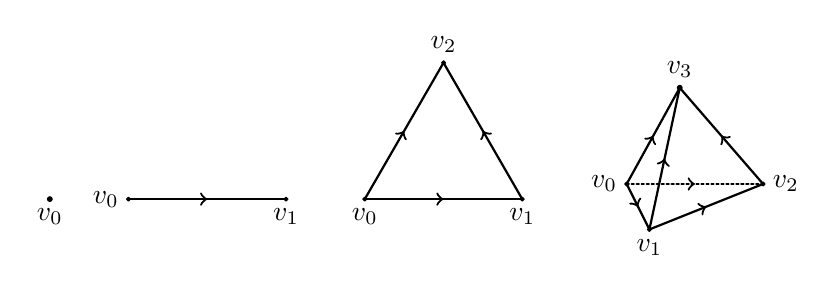
\begin{tikzpicture}[line join = round, line cap = round]

                        % 0-simplex
                        \coordinate [label=below:$v_0$] (0) at (0,0);
                        % 1-simplex
                        \coordinate [label=left:$v_0$] (1) at (1,0);
                        \coordinate [label=below:$v_1$] (2) at (3,0);
                        % 2-simplex
                        \coordinate [label=below:$v_0$] (3) at (4,0);
                        \coordinate [label=below:$v_1$] (4) at (6,0);
                        \coordinate [label=above:$v_2$] (5) at (5,{sqrt(3)});
                        % 3-simpex
                        \coordinate [label=above:$v_3$] (6) at (8,{sqrt(2)},0);
                        \coordinate [label=left:$v_0$] (7) at ({-.5*sqrt(3)+8},0,-.5);
                        \coordinate [label=below:$v_1$] (8) at (8,0,1);
                        \coordinate [label=right:$v_2$] (9) at ({.5*sqrt(3)+8},0,-.5);

                        \begin{scope}[decoration={markings,mark=at position 0.5 with
                            {\arrow{to}}}]
                            % 0-simplex
                            \draw[fill] (0) circle [radius=0.03];
                            % 1-simplex
                            \draw[fill] (1) circle [radius=0.025];
                            \draw[fill] (2) circle [radius=0.025];
                            \draw[thick, postaction={decorate}] (1)--(2);
                            % 2-simplex
                            \draw[fill] (3) circle [radius=0.025];
                            \draw[fill] (4) circle [radius=0.025];
                            \draw[fill] (5) circle [radius=0.025];
                            \draw[thick, postaction={decorate}] (3)--(4);
                            \draw[thick, postaction={decorate}] (3)--(5);
                            \draw[thick, postaction={decorate}] (4)--(5);
                            % 3-simplex
                            \draw[fill] (6) circle [radius=0.03];
                            \draw[fill] (7) circle [radius=0.025];
                            \draw[fill] (8) circle [radius=0.025];
                            \draw[fill] (9) circle [radius=0.025];
                            \draw[thick, densely dotted,postaction={decorate}] (7)--(9);
                            \draw[thick, postaction={decorate}] (7)--(8);
                            \draw[thick, postaction={decorate}] (7)--(6);
                            \draw[thick, postaction={decorate}] (8)--(9);
                            \draw[thick, postaction={decorate}] (8)--(6);
                            \draw[thick, postaction={decorate}] (9)--(6);
                        \end{scope}

                    \end{tikzpicture}
                    
             The boundary $\partial\Delta^n$ is defined as the union of all the faces of $\Delta^n$, and
             $\mathring{\Delta^n} = \Delta^n - \partial\Delta^n $ denotes interior of $\Delta^n$. 
             
		      \begin{defn}[$\Delta$-complex]
		      	A $\Delta-complex$ structure on a space X is a collection of maps $\sigma_\alpha: \Delta^n \rightarrow X $ , with n depending on the index $\alpha$, such that:
                    \begin{enumerate}
                        \item The restriction $\sigma_\alpha | \mathring{\Delta^n}$ is                      injective, and each point of X is in the image of exactly one such restriction $\sigma_\alpha | \mathring{\Delta^n}$.
                        \item Each restriction of $\sigma_\alpha$ to a face of $\Delta^n$ is one of the  maps
                        $\sigma_\beta: \Delta^{n-1} \rightarrow X $. Here we are identifying the face of $\Delta^n$ with $\Delta^{n-1}$ by the canonical linear homeomorphism between them that preserves the ordering of the vertices.
                        \item A set $A \subset X$ is open iff $\sigma^{-1}_{\alpha}(A)$ is open in $\Delta^n$ for each $\sigma_\alpha$
                    \end{enumerate}

		      \end{defn}
		      
		      ...........................
		      Some explicit examples of $\Delta$-complex structures on spaces. E.g., 
		      a closed interval $[0;1]$
		      $X=S^1$ with some \emph{explicit} maps from $\Delta^1$ (preferably several different ones) 
		      $S^2$ with some explicit maps. More examples on some quotient spaces, $S^1\times S^1$, $\RR\PP^2$, Klein bottle.
		      ................................
		      
        \begin{Ex}
        
        Consider $\sigma_\alpha: \Delta^n \rightarrow X $ where $ X = S^1 = \{ (x,y) \in \RR^2 \, | \, x^2 + y^2 = 1 \} $ \\
        
		     
		       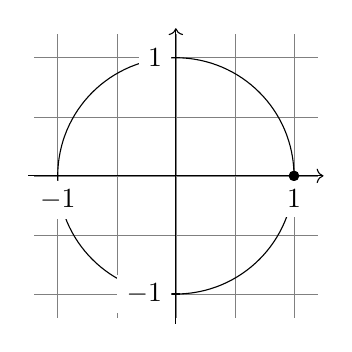
\begin{tikzpicture}[scale=1.5]
                \draw[step=.5cm, gray, very thin] (-1.2,-1.2) grid (1.2,1.2); 
                \draw[->] (-1.25,0) -- (1.25,0) coordinate (x axis);
                \draw[->] (0,-1.25) -- (0,1.25) coordinate (y axis);
                \draw (0,0) circle (1cm);
                \draw[fill] (1,0) circle (0.04);

                \foreach \x/\xtext in {-1, 1} 
                \draw (\x cm,1pt) -- (\x cm,-1pt) node[anchor=north,fill=white] {$\xtext$};
                \foreach \y/\ytext in {-1, 1} 
                \draw (1pt,\y cm) -- (-1pt,\y cm) node[anchor=east,fill=white] {$\ytext$};
                \end{tikzpicture}
              
              
		      For n = 0, $\alpha = 0$:  $\sigma_0: \Delta^0 \rightarrow S^1 $ where $\sigma_0(1) = (1, 0)$
		      
              For n = 1, $\alpha = 1$: In the figure below $t_0 + t_1 = 1$, $t_0, t_1 \geq 0$
              
              $ \Delta^1 = \{ (t_0, 1-t_0) \, , \, t_0 \in [0, 1] \} = [e_0, e_1] $ \\
              
              
             
              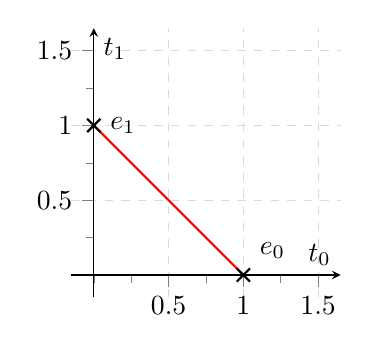
\begin{tikzpicture}
                    \tikzstyle{point}=[thick,draw=black,cross out,inner sep=0pt,minimum width=4pt,minimum height=4pt]
                    \begin{axis}[
                        legend pos=south west,
                        axis x line=middle,
                        axis y line=middle,
                        grid = major,
                        width=5cm,
                        height=5cm,
                        grid style={dashed, gray!30},
                        xmin=0,    % start the diagram at this x-coordinate
                        xmax=1.5,    % end   the diagram at this x-coordinate
                        ymin=0,    % start the diagram at this y-coordinate
                        ymax=1.5,    % end   the diagram at this y-coordinate
                        xlabel=$t_0$,
                        ylabel=$t_1$,
                        tick align=outside,
                        minor tick num=-3,
                        enlargelimits=true,
                        tension=0.08]
                    \addplot[domain=0:1, red, thick,samples=20] {-x+1};
                    \node[point,label={[label distance=0cm]45:$e_0$}] at (axis cs:1,0) {};
                    \node[point,label={[label distance=0cm]0:$e_1$}] at (axis cs:0,1) {};
                    \end{axis}
            \end{tikzpicture}

              $\sigma_1: \Delta^1 \rightarrow S^1 $ where $t_0 \in [0, 1]$ where $\sigma_1(t_0) = (\cos(2\pi t_0), \sin(2\pi t_0))$ \\
              $\sigma|_{[e_0]} = \sigma_1(0) = (\cos(0), \sin(0)) = (1, 0)$ \\
              $\sigma|_{[e_1]} = \sigma_1(1) = (\cos(2\pi), \sin(2\pi)) = (1, 0)$
              
     \end{Ex}

     \begin{Ex}
        
        Consider $\sigma_\alpha: \Delta^n \rightarrow X $ where $ X = S^2 = \{ (x,y,z) \in \RR^2 \, | \, x^2 + y^2 + z^2 = 1 \} $ \\
        
		     
		      
              
              
		      For n = 2, $\alpha = 2$:  $\sigma_2: \Delta^2 \rightarrow S^2 $
		      
              $ \Delta^1 = \{ (t_0, t_1, t_2) \, | \, t_0 + t_1 + t_2 = 1, \, t_i \geq 0 \; for \, i = 1, 2, 3] \} = [e_0, e_1, e_2] $ \\
            \tdplotsetmaincoords{70}{130}
            \begin{tikzpicture}[tdplot_main_coords, scale=2]
                    \def\laxis{2}
                    \def\ltriangle{1}
                    \def\ltick{.2}
                    %%% axes
                    \draw [->] (0,0,0) -- (\laxis,0,0) node [below] {$t_0$};
                    \draw [->] (0,0,0) -- (0,\laxis,0) node [right] {$t_1$};
                    \draw [->] (0,0,0) -- (0,0,\laxis) node [left] {$t_2$};
                    
                    \draw [->, ultra thick] (0,0,0) -- (\ltriangle,0,0) node [below] {$e_0$};
                    \draw [->, ultra thick] (0,0,0) -- (0,\ltriangle,0) node [right] {$e_1$};
                    \draw [->, ultra thick] (0,0,0) -- (0,0,\ltriangle) node [left] {$e_2$};
                    %%% axes ticks
                    \pgfmathtruncatemacro{\nticks}{floor(\laxis)-1}
                    \begin{scope}[
                        help lines,
                        every node/.style={inner sep=1pt,text=black}
                        ]
                        \foreach \coord in {1,...,\nticks} {
                        \draw (\coord,\ltick,0) -- ++(0,-\ltick,0) -- ++(0,0,\ltick)
                        node [pos=1,left] {\coord};
                        \draw (\ltick,\coord,0) -- ++(-\ltick,0,0) -- ++(0,0,\ltick)
                        node [pos=1,right] {\coord};
                        \draw (\ltick,0,\coord) -- ++(-\ltick,0,0) -- ++(0,\ltick,0)
                        node [at start,above right] {\coord};
                        }
                    \end{scope}
                    %%% figure
                    \filldraw [opacity=.33,red] (\ltriangle,0,0) -- (0,\ltriangle,0)
                    -- (0,0,\ltriangle) -- cycle;
            \end{tikzpicture}
              
            The faces are $[e_1, e_2]$ or $(0, t_1, t_2)$, where $t_1 + t_2 = 1$, \\
            $[e_0, e_2]$ or $(t_0, 0, t_2)$, where $t_0 + t_2 = 1$, \\
            $[e_0, e_1]$ or $(t_0, t_1, 0)$, where $t_0 + t_1 = 1$. \\
              
             
              

              $\sigma_2((t_0, t_1, t_2)) = \frac{(t_0, t_1, t_2)}{\sqrt(t_0^2 + t_1^2 + t_2^2)}$ \\ 
              $\sigma|_{[e_1, e_2]}(t_1, t_2) =\frac{(t_1, t_2)}{\sqrt(t_1^2 + t_2^2)}$, \quad
              $\sigma|_{[e_0, e_2]]}(t_0, t_2) =\frac{(t_0, t_2)}{\sqrt(t_0^2 + t_2^2)}$ , \quad
              $\sigma|_{[e_0, e_1]}(t_1, t_2) =\frac{(t_0, t_1)}{\sqrt(t_0^2 + t_1^2)}$ ,
     \end{Ex}

		    
		    
		      

		
		\section{Chain Complexes}
		
		      \begin{defn}[Chain complex]
		      	   Complex of abelian groups. Homology of a complex.\\
		      	   A chain complex is a sequencee of homomorphisms of abelian groups:
		      	   \[
                        \xymatrix{
                            {...}  \ar[r] & 
                            C_{n+1}  \ar[r]^{\partial_{n+1}} & 
                            C_n  \ar[r]^{\partial_n} & 
                            C_{n-1}  \ar[r]^{\partial_{n-1}} & 
                            {...}  \ar[r] & 
                            C_1  \ar[r]^{\partial_1} & 
                            C_0  \ar[r]^{\partial_0 = 0}
                            & 0 \\ }
                   \]
		      	   where \(\partial_n\partial_{n+1}=0\) for each n  in $\mathbb{Z}$. The equation
		      	   \(\partial_n\partial_{n+1}=0\) is equivalent to the inclusion $ \Ima\partial_{n+1} \subset \ker\partial_n $.
		      \end{defn}
		      
		      ...............
			    As a remark: complex of $R$-modules, for a commutative ring $R$.
			    
		      Chain complexes from a $\Delta$-complex structure: definining the differential and checking the $\partial^2=0$ property.
		      ............................
		       
		      The map $\partial_n$ for a $\Delta$-complex $\mathcal{X}$ is a boundary homomorphism 
		      $\partial_n: \Delta_n(\mathcal{X}) \rightarrow \Delta_{n-1}(\mathcal{X})$ where the action on a basis element of $\Delta_n(\mathcal{X})$ is: 
		      \[
		         \partial_n(\sigma_\alpha) = \sum\limits_i (-1)^i \sigma_\alpha | [v_0, ... ,\hat{v_i}, ... , v_n]
              \] 
            where the '\^{}' symbol denotes the absence of that vertex.
            
            \begin{Lemma}
             The composition $\partial^2=0$ below is zero 
             \[
                \xymatrix{
                    \Delta_n(X)  \ar[r]^{\partial_n} & 
                    \Delta_{n-1}(X)  \ar[r]^{\partial_{n-1}} & 
                    \Delta_{n-2}(X)   \\ }
             \]
            \end{Lemma}

            \emph{Proof}: For n = 3 :
             \[
                \xymatrix{
                    \Delta_3(X)  \ar[r]^{\partial_3} & 
                    \Delta_2(X)  \ar[r]^{\partial_2} & 
                    \Delta_1(X)   \\ }
             \]
             Let us proof that $\partial_2 \partial_3 = 0$: \\
             $\partial_3\sigma = \sum\limits_i (-1)^i \sigma | [v_0, ... ,\hat{v_i}, v_3] = 
             \sigma | [v_1, v_2, v_3] - \sigma | [v_0, v_2, v_3] + \sigma | [v_0, v_1, v_3] - \sigma | [v_0, v_1, v_2]$ \\
             
          
            \begin{equation}
                \begin{aligned}
                    \partial_2 \partial_3(\sigma) &= \sigma | [v_2, v_3] - \sigma | [v_1, v_3] + \sigma | [v_1, v_2] \\
                    &= -\sigma | [v_2, v_3] + \sigma | [v_0, v_3] - \sigma | [v_0, v_2] \\
                    &= \sigma | [v_1, v_3] - \sigma | [v_0, v_3] + \sigma | [v_0, v_1] \\
                    &= -\sigma | [v_1, v_2] + \sigma | [v_0, v_2] - \sigma | [v_0, v_1] = 0 
                \end{aligned}
            \end{equation}
            
        In case of n:
        
            \begin{equation}
                \begin{aligned}
                    \partial_{n-1} \partial_n(\sigma) &=  \partial_{n-1}(\sum\limits_i (-1)^i \sigma | [v_0, ... ,\hat{v_i}, ... , v_n]) \\
                    &=  \sum\limits_j (-1)^j ( \sum\limits_i (-1)^i \sigma | [v_0, ... ,\hat{v_i}, ... , v_n]) | [v_0, ... ,\hat{v_j}, ... , v_n] \\
                    &=  \sum\limits_{j<i} (-1)^i(-1)^j  \sigma_ | [v_0, ... ,\hat{v_j},... ,\hat{v_i} ... , v_n] +
                    \sum\limits_{j>i} (-1)^i(-1)^{j}  \sigma_ | [v_0, ... ,\hat{v_i},... ,\hat{v_j} ... , v_n] = 0
                \end{aligned}
            \end{equation}
		 
		 \section{Homology Calculations: Examples}
		 
		 $S^1$ with several different $\Delta$-complex structures. An interval $[0;1]$.
		 
		 
              \subsection{$ S^1$}
                \subsubsection{Method I: Triangulation}
                To compute the homolgy group of the circle $S^1$ we can triangulate the circle in the following way: \\
                
                        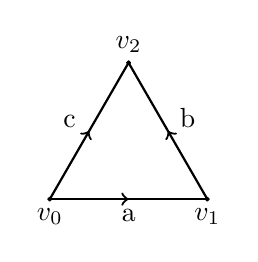
\begin{tikzpicture}[line join = round, line cap = round]
              
                                % 2-simplex
                                \coordinate [label=below:$v_0$] (3) at (4,0);
                                \coordinate [label=below:$v_1$] (4) at (6,0);
                                \coordinate [label=above:$v_2$] (5) at (5,{sqrt(3)});
                                
                                \begin{scope}[decoration={markings,mark=at position 0.5 with {\arrow{to}}}]
                                    
                                    \draw[fill] (3) circle [radius=0.025];
                                    \draw[fill] (4) circle [radius=0.025];
                                    \draw[fill] (5) circle [radius=0.025];
                                    \draw[thick, postaction={decorate}] (3)--(4) node [midway, below] {a};
                                    \draw[thick, postaction={decorate}] (3)--(5) node [near start, above=10pt] {c};
                                    \draw[thick, postaction={decorate}] (4)--(5) node [near start, above=10pt] {b};
                                    
                                \end{scope}

                        \end{tikzpicture}
                    
                    We can construct the following chain complex which is a sequence of homomorphisms of abelian groups: 

	\[
		\xymatrix{
			0  \ar[r]^{\partial_2 = 0} & 
			C_1  \ar[r]^{\partial_1} & 
			C_0  \ar[r]^{\partial_0 = 0}
			& 0 \\ }
	\]

 where \(\partial_n\partial_{n+1}=0\) for each n  in $\mathbb{Z}$ and 
 
			\[
				\left|
				  \begin{array}{l}
				  	C_0= \langle v_0, v_1, v_2 \rangle \\
				  	C_1=\langle a, b, c \rangle \\
                    C_n=\{0\} \quad \forall n \geqslant 2 
				  \end{array}
				\right., 
			\]

			\[
                \xymatrix{
                    0  \ar[r]^{\partial_2 = 0} & 
                    \mathbb{Z}^{\oplus^3}  \ar[r]^{\partial_1} & 
                    \mathbb{Z}^{\oplus^3}  \ar[r]^{\partial_0 = 0}
                    & 0 \\ }
	        \]
The n-th homology group is defined as $H_n = \frac{\ker\partial_n}{\Ima\partial_{n+1}}$. \\

\par
First, let's compute $H_0$: \\
$\ker\partial_0 = C_0 = \langle v_0, v_1, v_2 \rangle$ since $\partial_0 = 0$ \\ 
To calculate $\Ima\partial_1$, let's compute $\partial_1(\alpha a + \beta b + \gamma c) = \alpha (v_1-v_0) + \beta (v_2-v_1) - \gamma (v_2-v_0) \\ = (-\alpha + \gamma)v_0 + (\alpha - \beta)v_1 + (\beta - \gamma)v_2 = (\gamma -\alpha)v_0 + (\alpha - \beta)v_1 + (-(\gamma - \alpha)-(\alpha - \beta))v_2 $ \\
$\Ima\partial_1 = \left\{ \left(\begin{array}{c}
          		                 	( \gamma - \alpha )\\
          		                 	(\alpha - \beta)\\
          		                 	-(\gamma - \alpha)-(\alpha - \beta)\\
          		                 \end{array} \right), \quad \alpha, \beta, \gamma \subseteq \mathbb{Z} \right\} \subseteq \mathbb{Z}^{\oplus^3} $ \\
          		                 
$Claim: $ There exist an isomorphism $\psi: \Ima\partial_1 \simeq \mathbb{Z}^2$\\ 
$\psi: \left(\begin{array}{c}
                    ( \gamma - \alpha )\\
                    (\alpha - \beta)\\
                    (\beta - \gamma)\\
            \end{array} \right) \mapsto
            \left(\begin{array}{c}
                    ( \gamma - \alpha )\\
                    (\alpha - \beta)\\
            \end{array} \right)$ \\
$\psi $ is one-to-one since if $ ( \gamma - \alpha  = 0 \; \& \; \alpha - \beta = 0) \Rightarrow \beta - \gamma = 0  \; \& \; \alpha = \beta = \gamma $ \\
$\psi $ is onto since given $\left(\begin{array}{c}
                    m\\
                    n\\
            \end{array} \right) \in \mathbb{Z}^2$ 
        there exist an element $\left(\begin{array}{c}
                    m\\
                    n\\
                    -m-n\\
            \end{array} \right) \in \Ima\partial_1 $ such that \\
$\psi \left(\begin{array}{c}
                    m\\
                    n\\
                    -m-n\\
            \end{array} \right) = 
      \left(\begin{array}{c}
                    m\\
                    n\\
            \end{array} \right)$, since $\psi$ is one-to-one and onto, $\Ima\partial_1 \simeq \mathbb{Z}^2$ 

$H_0 = \frac{\ker\partial_0}{\Ima\partial_1} = \mathbb{Z}^{3} \left/ {
    \left(\begin{array}{c}
                    1\\
                    0\\
                    -1\\
            \end{array} \right)\mathbb{Z} \oplus
    \left(\begin{array}{c}
                    0\\
                    1\\
                    -1\\
            \end{array} \right)\mathbb{Z}} \right.$ \\

    Claim: $ \phi: \left( \mathbb{Z}^{3} \left/ {
    \left(\begin{array}{c}
                    1\\
                    0\\
                    -1\\
            \end{array} \right)\mathbb{Z} \oplus
    \left(\begin{array}{c}
                    0\\
                    1\\
                    -1\\
            \end{array} \right)\mathbb{Z}} \right. \right) \simeq \mathbb{Z}$ \\

            First, let us take the map $\varphi: \mathbb{Z}^{3} \rightarrow \mathbb{Z}^{3} \left/
            \left\langle \left( \begin{array}{c}
                    1\\
                    0\\
                    -1\\
            \end{array} \right), \left(\begin{array}{c}
                    0\\
                    1\\
                    -1\\
            \end{array} \right)  \right\rangle \right.$ \\
$\mathbb{Z}^{3} \ni  \left(\begin{array}{c}
                    p\\
                    q\\
                    r\\
            \end{array} \right) = 
            p\left(\begin{array}{c}
                    1\\
                    0\\
                    -1\\
            \end{array} \right) +
            q\left(\begin{array}{c}
                    0\\
                    1\\
                    -1\\
            \end{array} \right) + 
            (p+q+r)\left(\begin{array}{c}
                    0\\
                    0\\
                    1\\
            \end{array} \right) $ \\ where $ 
            p\left(\begin{array}{c}
                    1\\
                    0\\
                    -1\\
            \end{array} \right) +
            q\left(\begin{array}{c}
                    0\\
                    1\\
                    -1\\
            \end{array} \right) \in \left(\begin{array}{c}
                    1\\
                    0\\
                    -1\\
            \end{array} \right)\mathbb{Z} +
    \left(\begin{array}{c}
                    0\\
                    1\\
                    -1\\
            \end{array} \right)\mathbb{Z} $ \\
            
So, $\varphi: \left(\begin{array}{c}
                    p\\
                    q\\
                    r\\
            \end{array} \right) \mapsto \overline{\left(\begin{array}{c}
                    p\\
                    q\\
                    r\\
            \end{array} \right)} = (p+q+r) \overline{\left(\begin{array}{c}
                    0\\
                    0\\
                    1\\
            \end{array} \right)}$ \\

           Finally, $ \phi: \overline{\left(\begin{array}{c}
                    p\\
                    q\\
                    r\\
            \end{array} \right)} \mapsto (p+q+r) \in \mathbb{Z} $, Clearly, $\phi$ is injective and surjective. 
            
          So, $H_0 \simeq \mathbb{Z} $ \\

\par
Second, let's compute $H_1$: \\
$\ker\partial_1 = \left\{ \left(\begin{array}{c}
                    m\\
                    m\\
                    m\\
            \end{array} \right), m \in \mathbb{Z} = \right\} = \left(\begin{array}{c}
                    1\\
                    1\\
                    1\\
            \end{array} \right) \mathbb{Z} \simeq \mathbb{Z}$ \\ 
$\Ima\partial_2 = \{0\}$ since $C_2 = \{0\}$ \\
$H_1 = \frac{\ker\partial_1}{\Ima\partial_2} = 
		\frac{ \ker{\partial_1} }{ \{0\} } = \ker{\partial_1} \simeq \mathbb{Z}$ \\


Finally, the homology groups of the circle are: 
		\[
	  		H_n^\Delta(S^1) \simeq \left\{
			      \begin{array}{rl}
			     \mathbb{Z}, & \textrm{for} \: n = 0, 1\\
			    
                        0 & \textrm{for} \: n \geqslant 2
			      \end{array}
			 \right.
	  	\]

 \subsubsection{Method II}
                  To compute the homolgy group of the circle $S^1$ we can construct the circle, by two verteces and two edges, in the following way: \\
                
              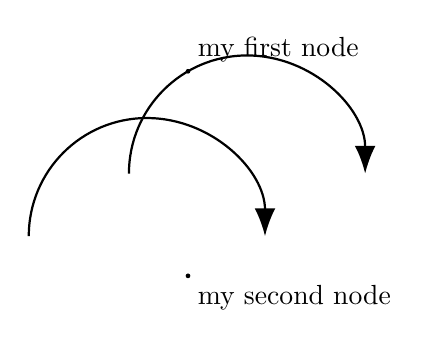
\begin{tikzpicture}[scale=1.5, >=latex, radius = 1]
                    \draw[thick, arrows = {-Latex[length=10]}]
                        (212:0) arc[start angle = 180, end angle = 0];
                    \draw[thick, arrows = {-Latex[length=10]}]
                        (212:1) arc[start angle = 180, end angle = 0];
                    \fill (60:1) circle[radius=0.02] node[above right] (n1) {my first node};
                    \fill (-60:1) circle[radius=0.02] node[below right] (n2) {my second node};

            \end{tikzpicture}
                       
                    We can construct the following chain complex which is a sequence of homomorphisms of abelian groups: 

	\[
		\xymatrix{
			0  \ar[r]^{\partial_2 = 0} & 
			C_1  \ar[r]^{\partial_1} & 
			C_0  \ar[r]^{\partial_0 = 0}
			& 0 \\ }
	\]

 where \(\partial_n\partial_{n+1}=0\) for each n  in $\mathbb{Z}$ and 
 
			\[
				\left|
				  \begin{array}{l}
				  	C_0= \langle v_0, v_1\rangle \\
				  	C_1=\langle a, b \rangle \\
                    C_n=\{0\} \quad \forall n \geqslant 2 
				  \end{array}
				\right., 
			\]

			\[
                \xymatrix{
                    0  \ar[r]^{\partial_2 = 0} & 
                    \mathbb{Z}^{\oplus^2}  \ar[r]^{\partial_1} & 
                    \mathbb{Z}^{\oplus^2}  \ar[r]^{\partial_0 = 0}
                    & 0 \\ }
	        \]
The n-th homology group is defined as $H_n = \frac{\ker\partial_n}{\Ima\partial_{n+1}}$. \\

\par
First, let's compute $H_0$: \\
$\ker\partial_0 = C_0 = \langle v_0, v_1 \rangle$ since $\partial_0 = 0$ \\ 
To calculate $\Ima\partial_1$, let's compute $\partial_1(\alpha a + \beta b) = \alpha (v_1-v_0) + \beta (v_1-v_0) = (\alpha + \beta)(v_1 - v_0)$  \\
$\Ima\partial_1 = \langle v_1 - v_0 \rangle$ \\
$H_0 = \frac{\ker\partial_0}{\Ima\partial_1} = \frac{ \langle v_0, v_1 \rangle  }{ \langle v_1-v_0 \rangle } = \frac{ \langle v_1-v_0, v_1 \rangle  }{ \langle v_1-v_0 \rangle }
                                                             =\langle v_1 \rangle  \simeq \mathbb{Z}$ \\

\par
Second, let's compute $H_1$: \\
$\ker\partial_1 = \left\{ \left(\begin{array}{c}
                    m\\
                    m\\
                    m\\
            \end{array} \right), m \in \mathbb{Z} = \right\} = \left(\begin{array}{c}
                    1\\
                    1\\
                    1\\
            \end{array} \right) \mathbb{Z} \simeq \mathbb{Z}$ \\ 
$\Ima\partial_2 = \{0\}$ since $C_2 = \{0\}$ \\
$H_1 = \frac{\ker\partial_1}{\Ima\partial_2} = 
		\frac{ \ker{\partial_1} }{ \{0\} } = \ker{\partial_1} \simeq \mathbb{Z}$ \\


Finally, the homology groups of the circle are: 
		\[
	  		H_n^\Delta(S^1) \simeq \left\{
			      \begin{array}{rl}
			     \mathbb{Z}, & \textrm{for} \: n = 0, 1\\
			    
                        0 & \textrm{for} \: n \geqslant 2
			      \end{array}
			 \right.
	  	\]

% ================================================================

               
		      \subsection{Torus}
      
One way to calculate the homology groups of a torus $T$ is by triangulating it into two 2-simplices A and B, upper triangle and lower one respectively.

	\[
		\xymatrix{
			v  \ar[r]^b \ar @{} [d]^(0.3) {\; A }
			& v \ar @{} [dl]^(0.55) {\; B} \\
			v \ar[u]^a \ar[r]_b \ar[ur]|{c}
			& v \ar[u]_a }
	\]
                                                                       
 We can construct the following chain complex which is a sequence of homomorphisms of abelian groups: 

	\[
		\xymatrix{
			0  \ar[r]^{\partial_3 = 0} & 
			C_2  \ar[r]^{\partial_2} & 
			C_1  \ar[r]^{\partial_1} & 
			C_0  \ar[r]^{\partial_0 = 0}
			& 0 \\ }
	\]

 where \(\partial_n\partial_{n+1}=0\) for each n  in $\mathbb{Z}$ and 
 
			\[
				\left|
				  \begin{array}{l}
				  	C_0= \langle v\rangle \\
				  	C_1=\langle a, b, c \rangle \\
                                C_2=\langle A, B \rangle \\
				      C_n=\{0\} \quad \forall n \geqslant 3 
				  \end{array}
				\right., 
			\]

			\[
                \xymatrix{
                    0  \ar[r]^{\partial_3 = 0} & 
                    \mathbb{Z}^{\oplus^2}  \ar[r]^{\partial_2} & 
                    \mathbb{Z}^{\oplus^3}  \ar[r]^{\partial_1} & 
                    \mathbb{Z}  \ar[r]^{\partial_0 = 0}
                    & 0 \\ }
	        \]
The n-th homology group is defined as $H_n = \frac{\ker\partial_n}{\Ima\partial_{n+1}}$. \\

\par
First, let's compute $H_0$: \\
$\ker\partial_0 = C_0 = \langle v \rangle$ since $\partial_0 = 0$ \\ 
$\Ima\partial_1 = \{0\}$ since $\partial_1(\alpha a + \beta b + \gamma c) = \alpha (v-v) + \beta (v-v) + \gamma (v-v) = 0 $ \\
$H_0 = \frac{\ker\partial_0}{\Ima\partial_1} = C_0 \simeq \mathbb{Z}$ \\

\par
Second, let's compute $H_1$: \\
$\ker\partial_1 = C_1 = \langle a,b,c \rangle$ 
		since $\partial_1 = 0$ \\ 
$\Ima\partial_2 = \langle a+b-c \rangle $ 
		since $\partial_2(\alpha A + \beta B) = \alpha (a+b-c) + \beta (a+b-c) = (\alpha + \beta) (a+b-c)$ \\
$H_1 = \frac{\ker\partial_1}{\Ima\partial_2} = 
		\frac{ \langle a,b,c \rangle  }{ \langle a+b-c \rangle }$ \\
The group $\langle a, b, c \rangle$ can be also generated by the elements 
		$ m=a+b-c, b \: and \: c $ where $a = m-b+c$. So, \\
$H_1 = \frac{\langle a+b-c,b,c \rangle }{ \langle a+b-c \rangle} = \langle b,c \rangle \simeq \mathbb{Z} \oplus \mathbb{Z} $ \\

\par
Last, let's compute $H_2$: \\
$\ker\partial_2 = \langle A-B \rangle$ 
		since $\partial_2(\alpha A + \beta B) = (\alpha + \beta) (a+b-c) = 0  \implies \alpha = -\beta$ so the kernel is generated by the element A-B \\
$\Ima\partial_3 = \{0\}$ since $C_3 = \{0\}$ \\ 
$H_2 = \frac{\ker\partial_2}{\Ima\partial_3} = 
		\frac{ \langle A-B \rangle  }{\{0\}} = \langle A-B \rangle \simeq \mathbb{Z}$ \\

Finally, the homology groups of the torus are: 
		\[
	  		H_n^\Delta(T) \simeq \left\{
			      \begin{array}{rl}
			     \mathbb{Z}, & \textrm{for} \: n = 0, 2\\
			     \mathbb{Z} \oplus \mathbb{Z}, & \textrm{for} \: n = 1\\
                        0 & \textrm{for} \: n \geqslant 3
			      \end{array}
			 \right.
	  	\]


% ================================================================



 		\subsection{$\mathbb{R} \mathbb{P}^2$}
      
One way to calculate the homology groups of a projective plain $\mathbb{R} \mathbb{P}^2$ is by triangulating it into two 2-simplices A and B, upper triangle and lower one respectively.

	\[
		\xymatrix{
			w \ar @{} [d]^(0.3) {\;\, A }
			& v  \ar[l]_b \ar[d]^a  \\
			v \ar[u]^a \ar[r]_b \ar[ur]|{c} 
			& w \ar @{} [u]^(0.3) {B \;\, } }
	\]
                                                                       
 We can construct the following chain complex which is a sequence of homomorphisms of abelian groups: 

    \[
		\xymatrix{
			0  \ar[r]^{\partial_3 = 0} & 
			C_2  \ar[r]^{\partial_2} & 
			C_1  \ar[r]^{\partial_1} & 
			C_0  \ar[r]^{\partial_0 = 0}
			& 0 \\ }
	\]
	
 where \(\partial_n\partial_{n+1}=0\) for each n  in $\mathbb{Z}$ and 
 
			\[
				\left|
				  \begin{array}{l}
				  	C_0=\langle v,w \rangle\\
				  	C_1=\langle a, b, c \rangle\\
                                C_2=\langle A, B \rangle\\
				      C_n=\{0\} \quad \forall n \geqslant 3 
				  \end{array}
				\right., 
			\]

    \[
		\xymatrix{
			0  \ar[r]^{\partial_3 = 0} & 
			\mathbb{Z}^{\oplus^2}  \ar[r]^{\partial_2} & 
			\mathbb{Z}^{\oplus^3}  \ar[r]^{\partial_1} & 
			\mathbb{Z}^{\oplus^2}  \ar[r]^{\partial_0 = 0}
			& 0 \\ }
	\]
The n-th homology group is defined as % $H_n = \frac{\ker\partial_n}{\Ima\partial_{n+1}}$.
$H_n= \ker\partial_n\left/ \Ima \partial_n \right. $\\

%\[
%	\ZZ\left/ 2\ZZ \right.
%\]


%\[
%	\left( \frac{1}{2}+\frac{4}{5} \right)
%\]


\par
First, let's compute $H_0$: \\
$\ker\partial_0 = C_0 = \langle v,w \rangle$ 
		since $\partial_0 = 0$ \\ 
$\Ima\partial_1 = \langle w-v \rangle$ 
		since $\partial_1(\alpha a + \beta b + \gamma c) = \alpha (w-v) + \beta (w-v) + \gamma (v-v)  \\ =(\alpha + \beta)(w-v) $ \\
$H_0 = \frac{\ker\partial_0}{\Ima\partial_1} = \frac{ \langle v, w \rangle  }{ \langle w-v \rangle } = \frac{ \langle w-v, w \rangle  }{ \langle w-v \rangle }
                                                             =\langle w \rangle  \simeq \mathbb{Z}$ \\

\par
Second, let's compute $H_1$: \\
$\ker\partial_1 = \langle a-b,c \rangle$ 
		since $\partial_1(\alpha a + \beta b + \gamma c) = (\alpha + \beta)(w-v) = 0  \implies \alpha = -\beta$ \\
The general element in $C_1$: $ (\alpha a + \beta b + \gamma c)= \alpha(a-b) + \gamma c $,
so the $\ker\partial_1$ can be generated by the elements a-b and c \\
$\Ima\partial_2 = \langle -a+b+c,\, a-b+c \rangle $ 
		since $\partial_2(\alpha A + \beta B) = \alpha(-a+b+c) + \beta(a-b+c)$ \\
$H_1 = \frac{\ker\partial_1}{\Ima\partial_2} = 
		\frac{ \langle a-b, \,c \rangle  }{ \langle -a+b+c,\, a-b+c \rangle }$\\
The group $\langle a-b, c \rangle$ can be also generated by the elements 
		$ m=a-b+c, and \: c $ where $ a - b = m -c $. So, \\
$H_1 = \frac{ \langle a-b, \,c \rangle  }{ \langle -a+b+c,\, a-b+c \rangle } = \frac{ \langle a-b+c, \, c \rangle  }{ \langle a-b+c,\, -a+b+c \rangle } $ \\
If we let $t=a-b+c$ then $-a+b+c = -t + 2c $ then the group $\langle t,\, -t+2c \rangle$ can be also generated by the elements $ t \: and \: 2c $. \\
In terms of t and c, $H_1 = \frac{ \langle t, \,c \rangle  }{ \langle t,\, 2c \rangle } = \frac{  \langle c \rangle  }{ \langle 2c \rangle } \simeq \frac{\mathbb{Z}}{2\mathbb{Z}}$ \\

\par
Last, let's compute $H_2$: \\
$\ker\partial_2 = \{0\}$ 
		since $\partial_2(\alpha A + \beta B) = (-\alpha+\beta)a +  (\alpha-\beta)b + (\alpha+\beta)c = 0 $ only when $\alpha = \beta = 0$\\
$\Ima\partial_3 = \{0\}$ since $C_3 = \{0\}$ \\ 
$H_2 = \frac{\ker\partial_2}{\Ima\partial_3} = 
		\frac{\{0\} }{\{0\}} = 0 $ \\

Finally, the homology groups of the projective plane are: 
		\[
	  		H_n^\Delta(\mathbb{R} \mathbb{P}^2) \simeq \left\{
			      \begin{array}{rl}
			     \mathbb{Z}, & \textrm{for} \: n = 0\\
			     \frac{\mathbb{Z}}{2\mathbb{Z}}, & \textrm{for} \: n = 1\\
                        0 & \textrm{for} \: n \geqslant 2
			      \end{array}
			 \right.
	  	\]


		
    \section{Maps of Complexes}
    \subsection{Maps on Homology}

		      
		      

 
 
 
 
 
 
 
 
 
 
 
 
\bibliographystyle{alpha}
\bibliography{biblio}
 
 

\end{document}          
